\documentclass[answers, a4paper, 11pt]{exam}
\usepackage{amsmath}
\usepackage{amssymb}
\usepackage{amsthm}
\usepackage[english]{babel}
\usepackage{ccicons}
\usepackage{hyperref}
\usepackage{cleveref}
\usepackage[utf8]{inputenc}
\usepackage[autostyle=false, style=english]{csquotes}
\usepackage[margin=2cm]{geometry}
\usepackage{graphicx}
\usepackage{mathrsfs}
\usepackage{multicol}
\usepackage{relsize}
\usepackage{parskip}
\usepackage{xcolor}
\pagestyle{plain}
\graphicspath{{./images/}}
\MakeOuterQuote{"}
\setlength{\columnseprule}{.4pt}
\renewcommand{\solutiontitle}{\noindent\textbf{R:}\enspace}
\def\dbar{{\mathchar'26\mkern-12mu d}}
\renewcommand{\thepartno}{\arabic{partno}}
\title{Virtual and Alternate Reality}
\author{Kevin Michael Frick}
\begin{document}
\maketitle
\begin{questions}
	\setcounter{question}{1}

	\question \textbf{VR systems}
	\begin{parts}
		\part Explain in which of the following cases an application can be considered as a Virtual Reality application and why:
		\begin{itemize}
			\item Interactive application with stereoscopic vision and tracking devices.
			\item A game for PC with very realistic images and scenes.
			\item A 3D animation movie with avatars created using very advanced design software.
			\item A game for a 3D TV with a Kinect as an input device.
		\end{itemize}
		\begin{solution}
			An interactive application with stereoscopic vision and tracking device, as well as a game for a three-dimensional television using a Kinect as an input device, can be considered VR applications.
			This is because they both provide three-dimensional immersion by substituting the visual information coming from the natural world with the ones provided through stereoscopic vision, as well as a way to implicitly interact with the environment by performing natural body movements that are tracked by the Kinect or other devices.

			A non-interactive three-dimensional movie or video game, however realistic, are clearly immersive experiences which however do not entirely substitute or augment the sensory information the user is receiving.
			In the case of the game, controls have to be given explicitly by interacting with a mouse and keyboard, and there is no substitution of the visual experience as the images are displayed on a screen that is clealy separate from the natural world.
			The case of the 3D animation movie is more complex, since the three-dimensional avatars could, in principle, effectively replace real images.
			However, the user is wholly aware that he or she is watching a movie, which provides no interaction and is therefore not as immersive as a virtual reality should be.
		\end{solution}
	\end{parts}
	\question \textbf{VR hardware}
	\begin{parts}
		\part Which 3D display technologies provide 3D stereoscopic images without breaking the natural accommodation/convergence relationship?
		\begin{solution}
			The Oculus Rift VR headset's lenses provide collimated light, therefore the eyes accommodate at infinity when wearing the headset.
			This means that the accommodation/convergence conflict is going to take place every time the user is looking at something that is not infinitely far away.

			The same conflict holds in the HTC Vive VR headset, where the eyes accommodate on a screen that is very close to the eye, but then converge on points whose depth is highly variable.

			Holographic (spinning mirror) displays can allow a single eye to focus on the virtual object in when the viewpoints are close enough to approximate a continuous 3D light field wavefront.
			This way, the depth cue of the virtual objects can be captured by the accommodation process of human eye, allowing it to accommodate on the virtual object and eliminating the accommodation/convergence conflict.

			Auto-stereoscopic displays are a textbook example of a device that breaks the accommodation/convergence relationship, since a point that is positioned at a different distance from the eyes than the screen is using stereoscopy causes the eyes to converge on that point while they are accommodating on the screen, thus causing vision decoupling.
		\end{solution}
		\part Indicate, for the following technologies, whether they require (Y) or not (N) electric power to work.
		\begin{itemize}
\item Polarizing glasses
\item Shutter glasses
\item Anaglyph glasses
\item Infitec glasses
		\end{itemize}
		\begin{solution}
			Anaglyph, Infitec and polarizing glasses are passive stereo technologies, so they do not require electric power to work; shutter glasses, on the other hand, need to be powered to alternate between opaque and transparent states for each lens and keep in sync with the display, via an infrared or wired signal.

		\end{solution}
		\part Considering the tracking of the Oculus Rift, describe how the acceleration data can be turned into positional data.
		\begin{solution}
			The Oculus Rift has an Inertial Measurement Unit (IMU) that reports angular velocity and linear acceleration.
			In order to get position from acceleration, two numerical integration steps have to be performed as shown:
			\begin{equation}
				\mathbf{v} = \int \mathbf{a} dt \implies \mathbf{s} = \int \mathbf{v} dt = \int \int \mathbf{a} dt dt
			\end{equation}

			These two steps magnify the measurement error in acceleration, eventually leading to position drift.
			In order to correct for this cumulative drift, data from a camera is used, which however has a much higher latency than the IMU (60 Hz vs 1000 Hz).
			For this reason, a combination of the two sensor is used in order to let the IMU estimate position via integration and then correct drift when camera position data is available.
		\end{solution}
	\end{parts}
	\question \textbf{Stereoscopic vision}
	\begin{parts}
		\part In a CAVE system, given a reference frame, how do you calculate inter-ocular distance, left-eye camera position, right-eye camera target inside that reference frame? How do you calculate the depth of a z-near clippling plane that guarantees no negative parallax?
		\begin{solution}
			The inter-ocular distance is simply the Euclidean distance betwen the two eyes.

			The position of a point in a given reference frame is given by left-multiplying the projection matrix (from world space to the desired reference frame) and the position vector of the point in world space.
			For example, we can assume the origin of world space to be in the middle of the cave, the Z axis pointing downwards, the X axis pointing to the right wall (looking from the top at the floor) and the Y axis looking in the opposite direction than the front wall.

			The translation matrix $\mathbf{T}$ is then defined as \begin{equation}
				\mathbf{T} = \begin{pmatrix}
					1 & 0 & 0 & F_x \\
					0 & 1 & 0 & F_y \\
					0 & 0 & 1 & F_z \\
					0 & 0 & 0 & 1
				\end{pmatrix}
			\end{equation}

			with $(F_x, F_y, F_z)$ being the position of the origin of the reference frame in world space.
			At this point, rotation matrices $\mathbf{R_x}, \mathbf{R_y}, \mathbf{R_z}$ that encode the rotation \emph{around} the $x, y, z$ axes, respectively.
			These have the form
			\begin{equation}
				\mathbf{R_x} = \begin{pmatrix}
					1 & 0 & 0 & 0 \\
					0 & \cos \theta_x & -\sin \theta_x & 0 \\
					0 & \sin \theta_x & \cos \theta_x & 0 \\
					0 & 0 & 0 & 1
				\end{pmatrix}
			\end{equation}

			\begin{equation}
				\mathbf{R_y} = \begin{pmatrix}
					\cos \theta_y & 0 & \sin \theta_y & 0 \\
					0 & 1 & 0 & 0 \\
					-\sin \theta_y & 0 & \cos \theta_y & 0 \\
					0 & 0 & 0 & 1
				\end{pmatrix}
			\end{equation}

			\begin{equation}
				\mathbf{R_z} = \begin{pmatrix}
					\cos \theta_z & -\sin \theta_z & 0 & 0 \\
					\sin\theta_z & \cos \theta_z & 0 & 0 \\
					0 & 0 & 1 & 0 \\
					0 & 0 & 0 & 1
				\end{pmatrix}
			\end{equation}

			Note that:

			\begin{itemize}
				\item the row and column corresponding to the axis of rotation is always the unit vector corresponding to that axis (e.g. $(1, 0, 0)$ for the $x$ axis)
				\item the cosine is always the first to appear when reading the matrix in either row-major or column-major order
				\item a sine and a cosine never appear in the same row or column
				\item a cosine is never negative
			\end{itemize}

			Once the translation and rotation matrices have been calculated, the projection matrix is then defined as $\mathbf{P} = \mathbf{T R_x R_y R_z}$. Note that the translation and rotation are sensitive to order, so they should be calculated one after the other, keeping this in mind.

			The target is defined by projecting the virtual camera onto the required screen.

			In order to avoid negative parallax, the z-near clipping plane has to lie on the screen where the projection is being done.

		\end{solution}

		\part Explain why accommodation and convergence depth cues can be in disagreement in some stereoscopic displays. Draw a figure to show the potential problem.
		\begin{solution}
			Both accommodation and convergence are depth cues that depend on the depth of the fixation point.
			Accommodation happens when the ciliary muscles of the eye induces deformation in the eye lens, or \emph{cristallino}, minimizing the amount of blur for the depth level of the part of the scene that we are fixating and allowing us to focus object at that level of depth.
			Convergence, on the other hand, happens when the eyeball rotates, allowing us to place the point being fixated on at the fovea, a point of the retina which is responsible for sharp central vision.
			In other words, accommodation is the focusing motion that happens by deforming the cristallino, while convergence is the turning inwards motion we feel when fixating on a close object.

			Normally, there is a natural relationship between accommodation and convergence.
			However, when looking at a screen, the images on the screen are located in different places.
			As a consequence, the location of the geometric image, seen stereoscopically, lies away from the plane of the screen.
			As shown in the following figure, the eyes accommodate on the screen, but converge on the location of the stereoscopic image, causing a conflict known as \emph{vision decoupling}.

			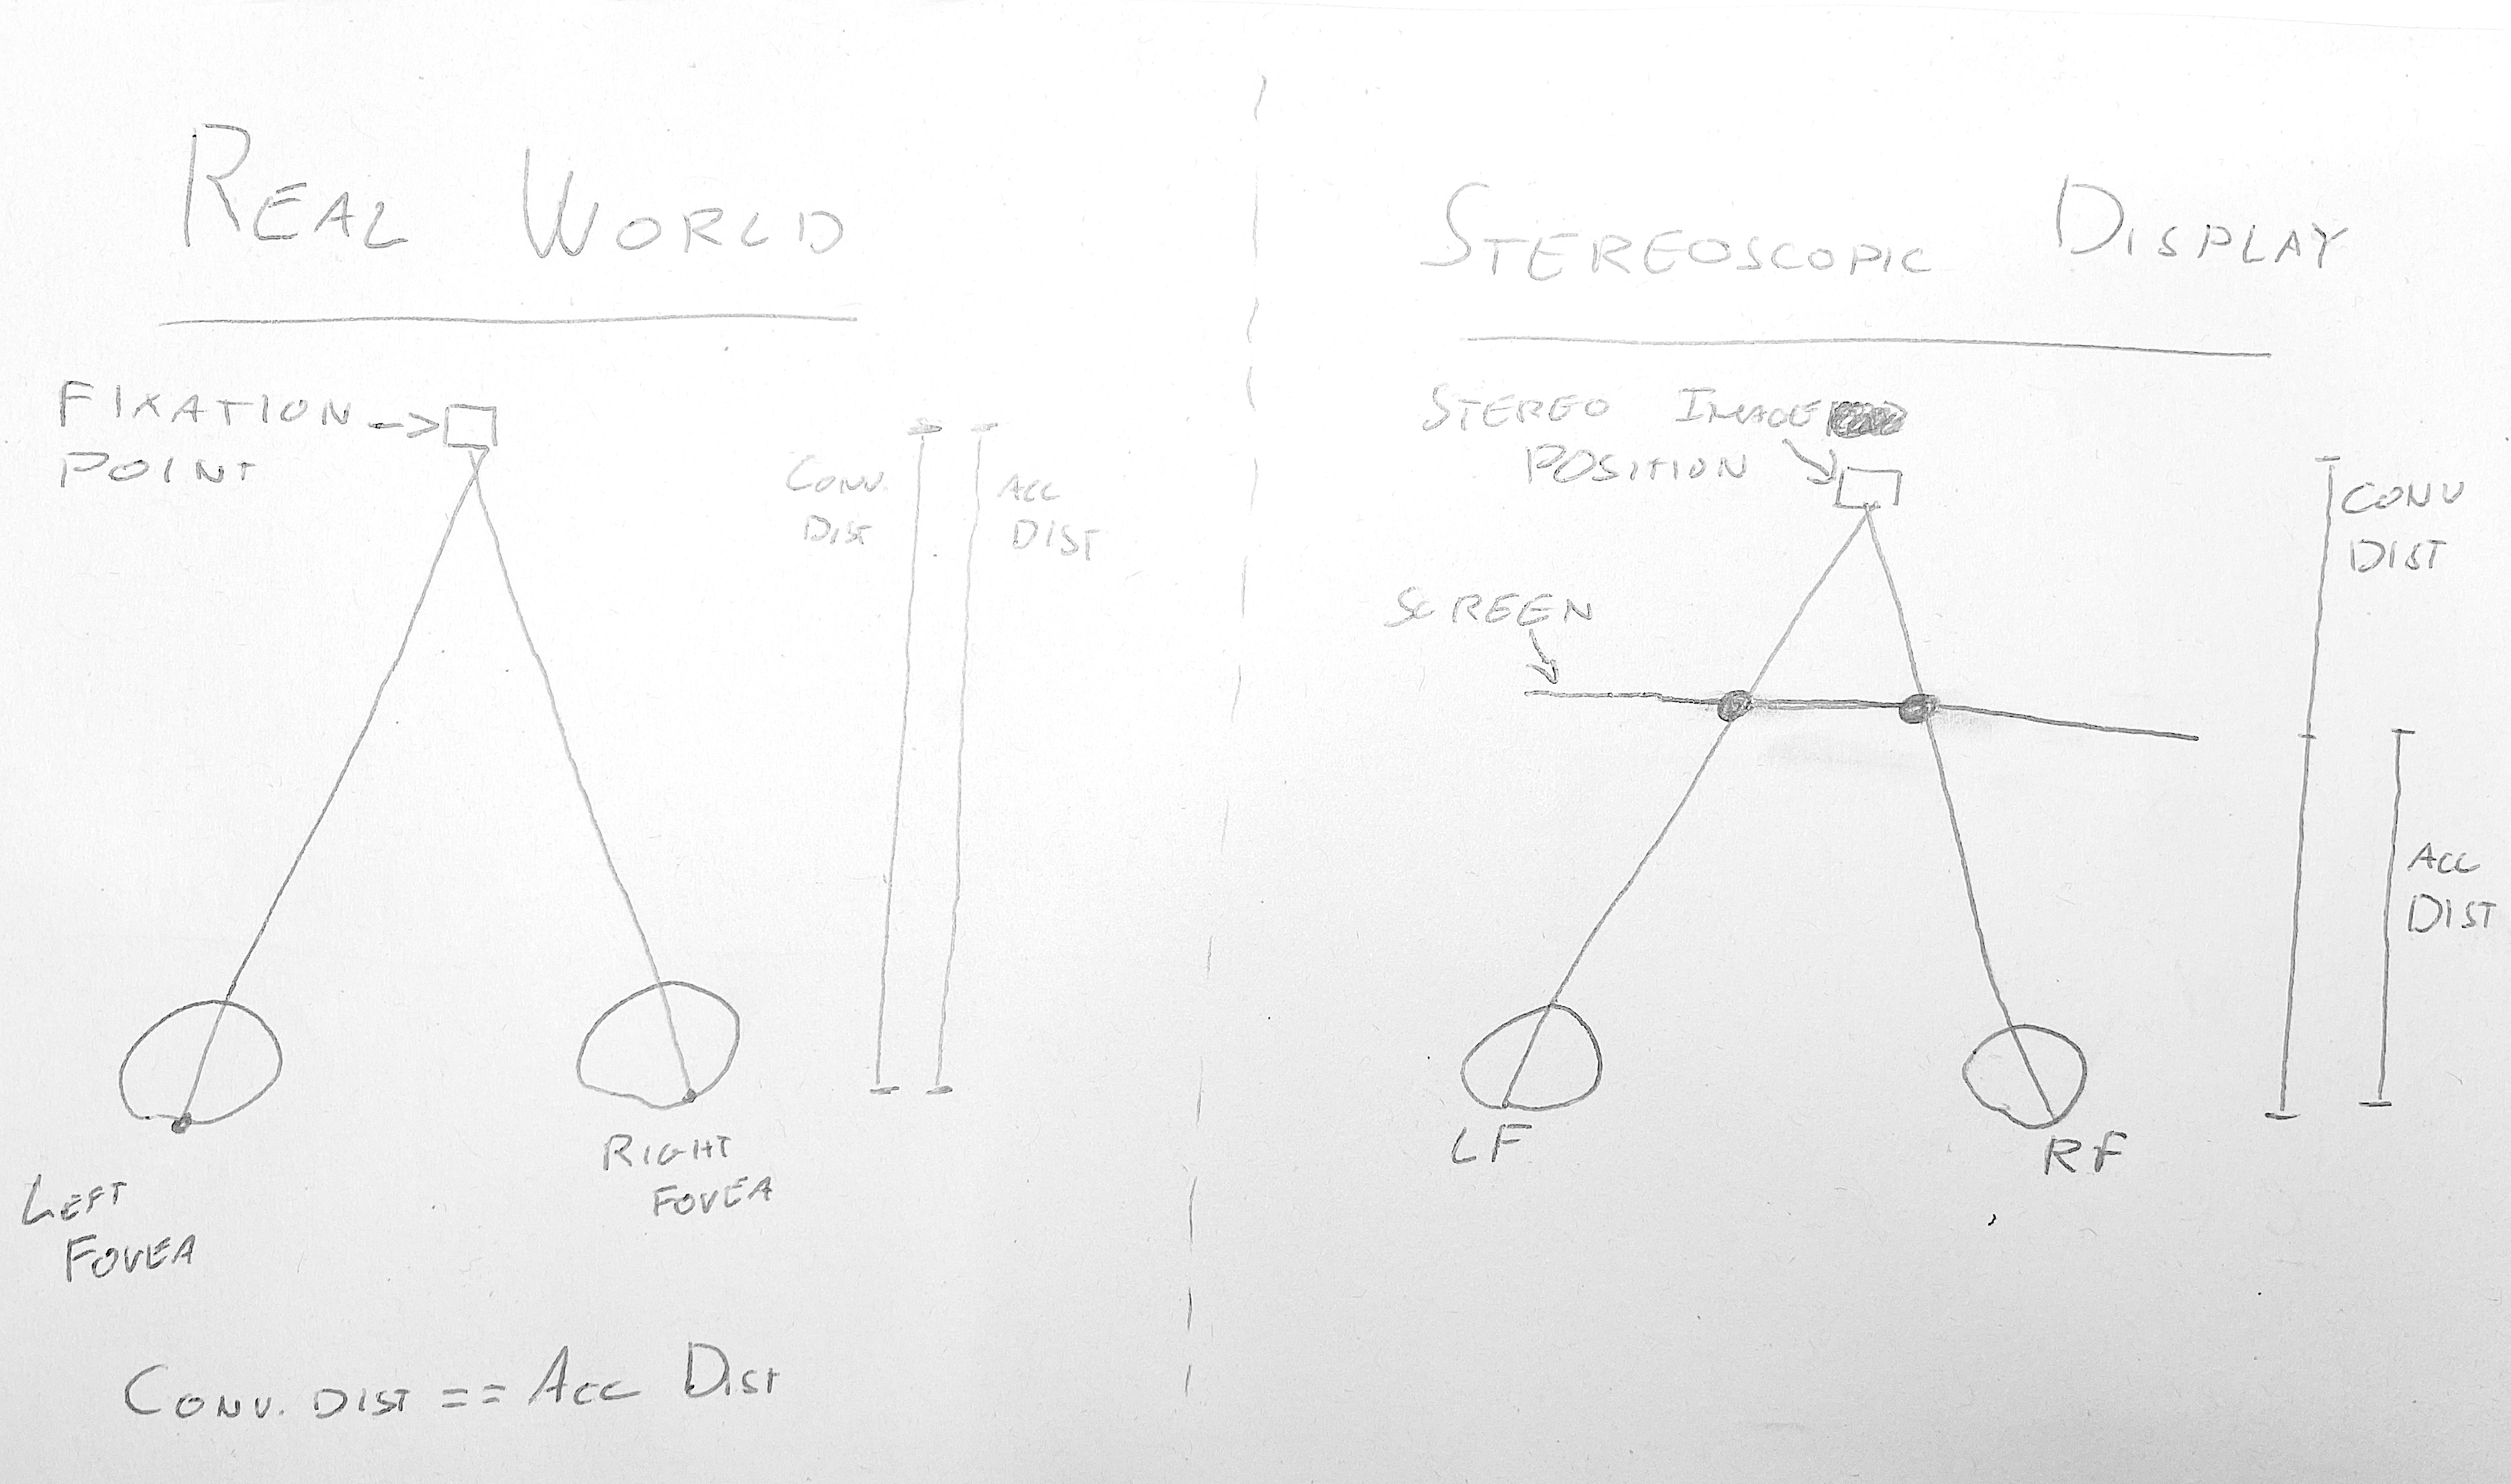
\includegraphics[width=\textwidth]{acc-vs-conv}

		\end{solution}
		\part Imagine two users looking exactly at the same fixation point from the same position, with the only difference that one user has an iod of 6cm and the other user has iod of 7cm. Would this difference affect their retinal disparity? Why?
		\begin{solution}
			On the fixation point, retinal disparity is zero regardless of IOD.
			For other points, inter-ocular distance is the very thing that determines the ratio between depth and retinal disparity.

			Disparity as a function of depth, IOD and focal length is defined by
			\begin{equation}
				disp(d, IOD, f) = \frac{f \cdot IOD}{d}
			\end{equation}

			therefore one user would have a retinal disparity equal to approximately $1.167$ times the other user.
		\end{solution}
		\part Imagine a VR application for protein inspection that can be used with and without head- tracking support.
		An experiment reveals that, when using head-tracking, people get a deeper knowledge of the spatial structure of the protein.
		Explain, \textbf{in terms of depth cues}, why this result could be expected.
		\begin{solution}
	Users can use the sensory cues provided by head movement to enhance the perception of 3D motion.
			Indeed, whole-body movements of an observer relative to a visual scene provide motion parallax cues that signal object depth.
			When the observer moves, the retinal images of objects close to the eye are displaced more quickly—and through a larger angle—than are the retinal images of more distant objects.

			Assuming that all the other depth cues that rely on position tracking - occlusion, shadowing, binocular parallax, etc. are implemented without the need for head tracking, for example via simpler body tracking and using stereo glasses, motion parallax then becomes one additional depth cue that can only be accurately calculated using head tracking.

		\end{solution}
	\end{parts}
	\question \textbf{Haptic rendering}
	\begin{parts}
		\part
	\end{parts}
	\question \textbf{VR software development}
	\begin{parts}
		\part
	\end{parts}
	\question \textbf{AR software development}
	\begin{parts}
		\part Answer the following questions with TRUE or FALSE:
		\begin{itemize}
			\item Using AR-Toolkit the application is able to recognize any image markers.
			\item Vuforia allows an AR application to recognize user defined targets as markers.
			\item An AR video see-through device can achieve the same resolution of the real world than an optical see-through device.
			\item The occlusion problem between real and virtual objects can be well supported in video see- through devices.
			\item A typical program using AR-Toolkit draws the virtual objects before the background video.
			\item In AR applications using hand-held displays, the stereoscopy is not the main objective.
		\end{itemize}
		\begin{solution}
			NOT INCLUDED IN THE MIDTERM.
		\end{solution}
	\end{parts}
	\question \textbf{3D user interfaces}
	\begin{parts}
		\part Indicate how selection and manipulation can be performed when using a virtual pointer.
		Provide details about the advantages and limitations for each of those two tasks.
		\begin{solution}
			Virtual pointers allow users to select and manipulate objects that are beyond the immediate reach of their limbs.
			It is a very suitable technique for selection, but manipulation is problematic since only radial movements can be made, which is bad for changing distance to the user.
			It's also a technique that is only effective for one degree of freedom, the axis of the pointer itself.
			Pointing should therefore be used for selection, while a virtual hand is better for manipulation.

			There are six metaphors for virtual pointers: ray casting, two-handed pointing, fishing reel, aperture, flashlight and image plane.

			When using ray casting, a line segment is attached to the hand and defines the pointing direction.
			This is a very precise technique as the selection volume is a single ray, but it presents problems in selecting objects that are far away.
			There are many variants: rays can be bent, or snap to the nearest object etc.
			A variant of ray casting is two-handed pointing, which requires two hands to be tracked in order to allow one to define the origin and the other to specify where the ray should point to.

			The fishing reel technique is similar to ray casting, but introduces an additional input device which controls the length of the virtual ray.

			Another metaphor is the flashlight, in which the selection volume is a cone, just like the light in a flashlight.
			The apex of the cone is defined by the position of the user's hand while the axis is its orientation.
			The aperture of the cone is constant.
			One issue that is immediately apparent with this metaphor is deciding which object to select when the cone comprises multiple objects.
			A possible rule is to select the object that is closest to the axis of the cone, but the issue still stands when the environment is very cluttered.
			A variant of the flashlight metaphor is using a cone whose axis points to the user's hand and whose axis is the line passing by the user's hand and eye.
			This way, aperture can be controlled by moving the sensor closer and device twist can be used to disambiguate between objects.

			The fishing reel technique is similar to ray casting, but introduces an additional input device which controls the length of the virtual ray.



		\end{solution}
	\end{parts}
	\question \textbf{Presence}
	\begin{parts}
		\part Of the following sentences, regarding presence in virtual environments, indicate which ones are TRUE and which ones are FALSE.
		\begin{itemize}
			\item Higher latency results in higher levels of presence.
			\item Walk in place results in higher presence than using a joystick in VE.
			\item Ray Tracing reports higher levels of presence than OpenGL illumination model.
			\item Heart rate and galvanic skin response are objective methods to measure presence.
		\end{itemize}
		\begin{solution}
			Presence is operationally defined as the successful substitution of real sensory data by computer-generated sense data.
			A ``successful'' response is realistic, similar to a real response.
			Here we are dealing with a low-level physiological response paving the way for higher-level cognitive and emotional responses which include verbal confirmations of ``being there''.

			Presence can be measured with physiological measures, such as heart rate and galvanic skin response.

			Navigating a virtual environment using a controller breaks the correlation between proprioception and sensory data, while experimental data confirms this doesn't happen with walking-in-place if the users associate well with their virtual bodies.

			Lower latency also results in a higher heart reate, which correlates with higher presence.

			Finally, experiments also confirms that ray tracing leads to higher presence than the OpenG illumination model.



		\end{solution}
		\part What are static haptics, and how can they enhance presence in virtual environments? Provide one example.
		\begin{solution}
			Passive haptics are a way of augmenting a high-fidelity visual virtual environment with low-fidelity physical objects that prevent the virtual bodies of users from passing through objects.
			Passive haptics do not replicate such properties as texture, thermal conductivity, and mass, nor do they replicate fine geometric details of the visual objects such as handles on cabinet drawers.
			Examples of static haptics are head-mounted displays and simple versions of physical objects.

			Adding physical objects will improve virtual environments because they make the objects feel to the user as if the objects are there. Humans can test the reality of an image by trying to touch the object, so if there is a real object where the users expects there to be one, presence (as measured with heart rate) is increased.

			One experiment investigated passive haptics's effects on performance of a real-world navigation task after training in a virtual environment.
 Half of the participants trained on maze navigation in a VE augmented with a styrofoam physical model, while half trained in a non-augmented VE but were given visual and audio contact cues.
 The task was to gain as much information as possible about the layout of the environment.
 Participants knew before the VE session that their training would be tested by navigating an identical real maze environment while blindfolded.

		\end{solution}
	\end{parts}

\end{questions}

\textbf{Disclaimer}:  This document may contain errors and inaccuracies that may damage your system, cause your partner to leave you, your boss to fire you, your cats to pee on your furniture and clothing, and global thermonuclear war. Proceed with caution. This document is released under the CC-BY-SA 4.0 license. \ccbysa
\end{document}
